% \documentclass{beamer}
% \usepackage{graphicx}
% \usepackage{multicol}
% \setlength{\columnseprule}{1pt}

% \graphicspath{{./fig/}}
% \usetheme{material}
% %%%%%%%%%%%%%%%%%%%%%%%%%%%%%%%%%%%%%%%%%%%%%%%%%%%%%%%%%%%%%%%%%%%%%%%%%%%%%%
% \embedvideo{<poster or text>}{<video file (MP4+H264)>}
% \embedvideo*{...}{...}                     % auto-play
%%%%%%%%%%%%%%%%%%%%%%%%%%%%%%%%%%%%%%%%%%%%%%%%%%%%%%%%%%%%%%%%%%%%%%%%%%%%%%

\ExplSyntaxOn
\NewDocumentCommand\embedvideo{smm}{
  \group_begin:
  \leavevmode
  \tl_if_exist:cTF{file_\file_mdfive_hash:n{#3}}{
    \tl_set_eq:Nc\video{file_\file_mdfive_hash:n{#3}}
  }{
    \IfFileExists{#3}{}{\GenericError{}{File~`#3'~not~found}{}{}}
    \pbs_pdfobj:nnn{}{fstream}{{}{#3}}
    \pbs_pdfobj:nnn{}{dict}{
      /Type/Filespec/F~(#3)/UF~(#3)
      /EF~<</F~\pbs_pdflastobj:>>
    }
    \tl_set:Nx\video{\pbs_pdflastobj:}
    \tl_gset_eq:cN{file_\file_mdfive_hash:n{#3}}\video
  }
  %
  \pbs_pdfobj:nnn{}{dict}{
    /Type/RichMediaInstance/Subtype/Video
    /Asset~\video
    /Params~<</FlashVars (
      source=#3&
      skin=SkinOverAllNoFullNoCaption.swf&
      skinAutoHide=true&
      skinBackgroundColor=0x5F5F5F&
      skinBackgroundAlpha=0
    )>>
  }
  %
  \pbs_pdfobj:nnn{}{dict}{
    /Type/RichMediaConfiguration/Subtype/Video
    /Instances~[\pbs_pdflastobj:]
  }
  %
  \pbs_pdfobj:nnn{}{dict}{
    /Type/RichMediaContent
    /Assets~<<
      /Names~[(#3)~\video]
    >>
    /Configurations~[\pbs_pdflastobj:]
  }
  \tl_set:Nx\rmcontent{\pbs_pdflastobj:}
  %
  \pbs_pdfobj:nnn{}{dict}{
    /Activation~<<
      /Condition/\IfBooleanTF{#1}{PV}{XA}
      /Presentation~<</Style/Embedded>>
    >>
    /Deactivation~<</Condition/PI>>
  }
  %
  \hbox_set:Nn\l_tmpa_box{#2}
  \tl_set:Nx\l_box_wd_tl{\dim_use:N\box_wd:N\l_tmpa_box}
  \tl_set:Nx\l_box_ht_tl{\dim_use:N\box_ht:N\l_tmpa_box}
  \tl_set:Nx\l_box_dp_tl{\dim_use:N\box_dp:N\l_tmpa_box}
  \pbs_pdfxform:nnnnn{1}{1}{}{}{\l_tmpa_box}
  %
  \pbs_pdfannot:nnnn{\l_box_wd_tl}{\l_box_ht_tl}{\l_box_dp_tl}{
    /Subtype/RichMedia
    /BS~<</W~0/S/S>>
    /Contents~(embedded~video~file:#3)
    /NM~(rma:#3)
    /AP~<</N~\pbs_pdflastxform:>>
    /RichMediaSettings~\pbs_pdflastobj:
    /RichMediaContent~\rmcontent
  }
  \phantom{#2}
  \group_end:
}
\ExplSyntaxOff

% \newlength{\wdth}

% \newcommand{\strike}[1]{\settowidth{\wdth}{#1}\rlap{\rule[.5ex]{\wdth}{.4pt}}#1}


% \begin{document}

\begin{frame}[label=real-31]{Since 1989, \ldots }
    \centering\cardImg{eth_zurich_3d_ptv_1989}{\textwidth}
\end{frame}

    
\begin{frame}[label=real-3]{3D PTV \strike{is} was a lab system}
    \centering\cardImg{lab.jpg}{.9\textwidth}
\end{frame}

\begin{frame}[label=real-4]{The time-resolved recording requires literally ``heavy lift''}
\begin{multicols}{2}
    \cardImg{ptv_drives1}{.495\textwidth}
    \cardImg{ptv_drives2}{.495\textwidth}
\end{multicols}
\end{frame}


% \begin{frame}[label=real-5]{We had a dream: 3D-PTV for large scale systems}
% \centering\cardImg{car_ptv.png}{.8\textwidth}
% \end{frame}

% \subsubsection*{Real time image acquisition and processing}
%\begin{frame}{The solution}
%\begin{card}
%\end{card}
%\end{frame}


\begin{frame}[label=real-66]{The bottlenecks for 1 min run at 1 kHz}
\begin{card}[Data transfer rate and size]
\begin{itemize}
\item 1.3 Mb/frame $\times$ 1000 frames/sec = 1300 Mb/sec
\item 1300 Mb/s $\times$ 4 cameras = 5.2 Gb/sec
\item SSD disk continuous writing speed is about 3.5 Gb/sec
\item Total data size: 5.2 Gb/sec $\times$ 60 $\approx$ 300 Gb
\end{itemize}

\end{card}
\end{frame}

\begin{frame}[label=real-6]{Need to eliminate the transfer rate bottleneck}
%\begin{card}[from compression to on-camera processing]
\begin{multicols*}{2}
\cardImg{realtime1}{.49\textwidth}
\cardImg{voth}{.48\textwidth}
%
\cardImg{mikrotron_sobel}{.49\textwidth}
\cardImg{mikrotron_inside}{.49\textwidth}
\end{multicols*}
%\end{card}
\end{frame}

\begin{frame}[label=real-7]{Sobel edge detection based algorithm}
\centering
\cardImg{sobel_1}{.8\textwidth}
\end{frame}


\begin{frame}[label=real-8]{Works very well for lab experiments}
\begin{card}
\centering
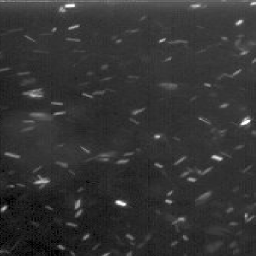
\includegraphics[width=.32\textwidth]{1_in}
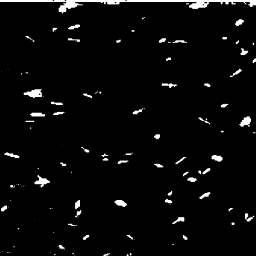
\includegraphics[width=.32\textwidth]{1_binarized}
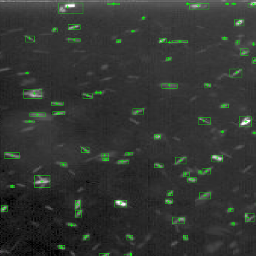
\includegraphics[width=.32\textwidth]{1_out}
\end{card}
\vspace{-.5cm}
\begin{cardTiny}
Raw image - binary image - blobs marked on the original image.  
\end{cardTiny}
\end{frame}


\begin{frame}[label=real-13]{Real life is not like this}
\begin{multicols}{2}
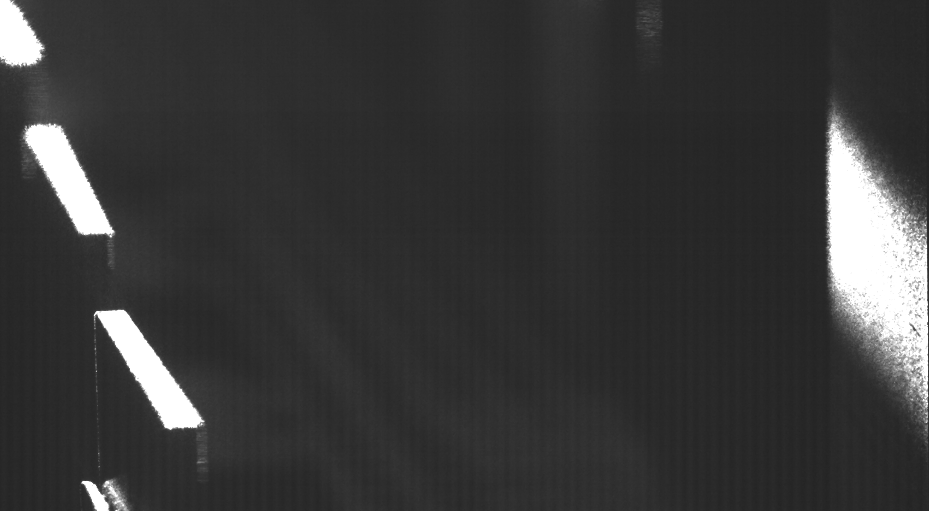
\includegraphics[width=.49\textwidth]{background.png}
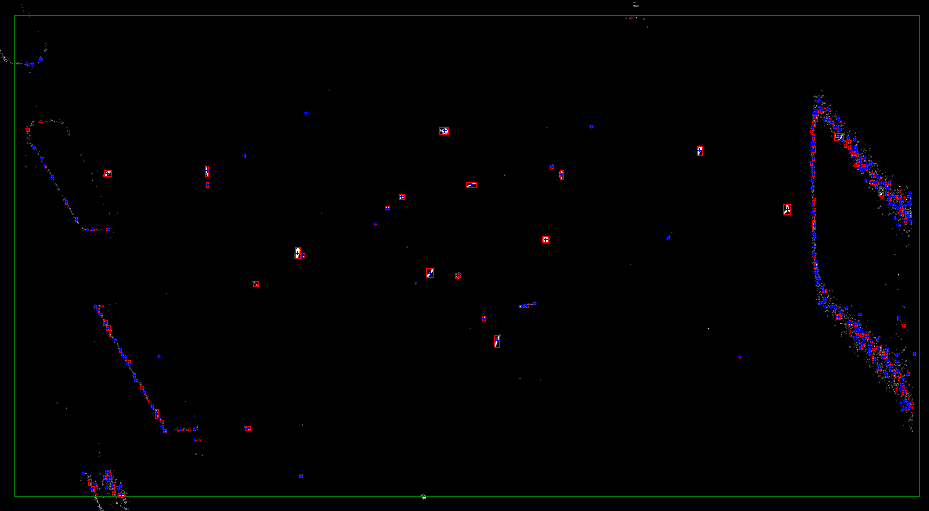
\includegraphics[width=.49\textwidth]{detection.png}
\end{multicols}
\begin{cardTiny}
Raw 3D-PTV image of the wind tunnel experiments: Background ->  binary image after background subtraction, and detection using a locally adaptive filter
\end{cardTiny}
\end{frame}

\begin{frame}[label=real-12]{We had to develop the know-how}
\centering\cardImg{1vision}{1\textwidth}
\end{frame}


\begin{frame}[label=real-11]{Image processing algorithm on FPGA}
\centering\cardImg{fig8}{1\textwidth}
% \begin{cardTiny} Diagram of the blob analysis algorithm. \end{cardTiny}
\end{frame}

\begin{frame}[label=real-10]{And its implementation on dedicated hardware}
\cardImg{1vision_blob_recorder_2}{1\textwidth}
% \cardImg{backside}{.25\textwidth}
\end{frame}

\begin{frame}[label=real-100]{The central concept diagram}
\centering
\cardImg[height=.8\textheight]{fig1.png}{\textwidth}
\end{frame}

%\end{document}